%%%%%%%%%%%%%%%%%%%%%%%%%%%%%%%%%%%%%%%%%%%%%%%%%%%%%%%%%%%%%%%%%%%%%%%%%%%%%%%%
%
% Fig 1: Histogram of percentage of explained of GWAS
%
%%%%%%%%%%%%%%%%%%%%%%%%%%%%%%%%%%%%%%%%%%%%%%%%%%%%%%%%%%%%%%%%%%%%%%%%%%%%%%%%

\begin{figure}[h!]
    \centering
    %
    \includegraphics[width=\textwidth]{\floatRelativePath/plthst_perc_tophits_eqtl.py/hist_perc_tophits_eqtl_excl_mhc.png}
    %
    \caption{}
    %
\end{figure}

%%%%%%%%%%%%%%%%%%%%%%%%%%%%%%%%%%%%%%%%%%%%%%%%%%%%%%%%%%%%%%%%%%%%%%%%%%%%%%%%
%
% Fig 2: Trait distance matrix
%
%%%%%%%%%%%%%%%%%%%%%%%%%%%%%%%%%%%%%%%%%%%%%%%%%%%%%%%%%%%%%%%%%%%%%%%%%%%%%%%%

\begin{figure}[h!]
    %
    \centering
    %
    \includegraphics[width=\textwidth]{\floatRelativePath/plthtmp_disease_comorbidity_matrix.py/corr_inkscape.png}
    %
    \caption{}
    %
\end{figure}

%%%%%%%%%%%%%%%%%%%%%%%%%%%%%%%%%%%%%%%%%%%%%%%%%%%%%%%%%%%%%%%%%%%%%%%%%%%%%%%%
%
% Fig 2: Length histogram of regions
%
%%%%%%%%%%%%%%%%%%%%%%%%%%%%%%%%%%%%%%%%%%%%%%%%%%%%%%%%%%%%%%%%%%%%%%%%%%%%%%%%

% \begin{figure}[!tbp]
% \centering
% %
% \begin{subfigure}[]{.33\textwidth}
% \textbf{a}
% \\
% \includegraphics[width=\textwidth]{\floatRelativePath/cmpt_pleiotropic_regions.py/regions_100000_length_hist.png}
% \end{subfigure}
% %
% \begin{subfigure}[]{.33\textwidth}
% \textbf{b}
% \\
% \includegraphics[width=\textwidth]{\floatRelativePath/pltbar_pleiotropic_regions_cumsum.py/pltbar_regions_cumsum.png}
% \end{subfigure}
% %
% \caption{Analysis of pleiotropic regions. \textbf{a}, Length distribution of pleiotropic regions. \textbf{b}, Cumulative sum ordered inversely with the number of GWAS classes.} \label{fig:pleiotropy_region_distribution}
% \end{figure}

%%%%%%%%%%%%%%%%%%%%%%%%%%%%%%%%%%%%%%%%%%%%%%%%%%%%%%%%%%%%%%%%%%%%%%%%%%%%%%%%
%
% Fig 3: Histograms of variants vs GWAS, eQTL genes and eQTL biosamples
%
%%%%%%%%%%%%%%%%%%%%%%%%%%%%%%%%%%%%%%%%%%%%%%%%%%%%%%%%%%%%%%%%%%%%%%%%%%%%%%%%

\begin{figure}[h!]
    %
    \centering
    %
    \begin{subfigure}[]{.32\textwidth}
        \textbf{a}
        \\
        \includegraphics[width=\textwidth]{\floatRelativePath/plthst_gwas_egene_etissue.py/hist_gwas.png}
    \end{subfigure}
    %
    \begin{subfigure}[]{.32\textwidth}
        \textbf{b}
        \\
        \includegraphics[width=\textwidth]{\floatRelativePath/plthst_gwas_egene_etissue.py/hist_egene.png}
    \end{subfigure}
    %
    \begin{subfigure}[]{.32\textwidth}
        \textbf{c}
        \\
        \includegraphics[width=\textwidth]{\floatRelativePath/plthst_gwas_egene_etissue.py/hist_etissue.png}
    \end{subfigure}
    %
    \caption{}
    %
\end{figure}

%%%%%%%%%%%%%%%%%%%%%%%%%%%%%%%%%%%%%%%%%%%%%%%%%%%%%%%%%%%%%%%%%%%%%%%%%%%%%%%%
%
% Fig 4: Spearman correlation between counts of GWAS categories, eQTL genes and eQTL biosamples
%
%%%%%%%%%%%%%%%%%%%%%%%%%%%%%%%%%%%%%%%%%%%%%%%%%%%%%%%%%%%%%%%%%%%%%%%%%%%%%%%%

\begin{figure}[h!]
    %
    \centering
    %
    \includegraphics[width=\textwidth]{\floatRelativePath/cmpt_count_per_rsid.py/count_per_rsid_gwas_egene_etissue_corr.png}
    %
    \caption{}
    %
\end{figure}

%%%%%%%%%%%%%%%%%%%%%%%%%%%%%%%%%%%%%%%%%%%%%%%%%%%%%%%%%%%%%%%%%%%%%%%%%%%%%%%%
%
% Fig 5: VEP consequences
%
%%%%%%%%%%%%%%%%%%%%%%%%%%%%%%%%%%%%%%%%%%%%%%%%%%%%%%%%%%%%%%%%%%%%%%%%%%%%%%%%

\begin{figure}[h!]
    %
    \centering
    %
    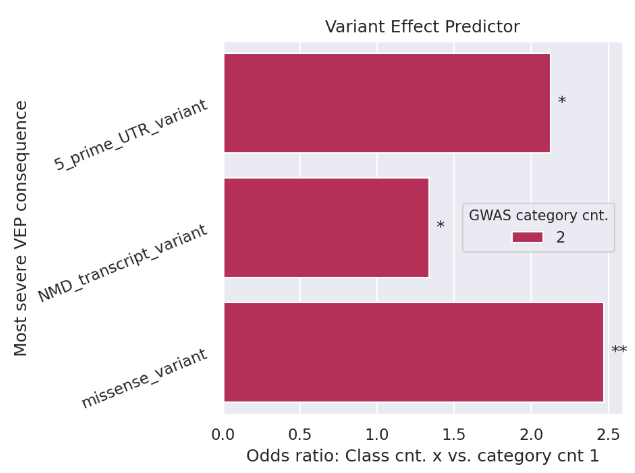
\includegraphics[width=\textwidth]{\floatRelativePath/pltbar_vep_consequence.py/vep.png}
    %
    \caption{}
    %
\end{figure}

%%%%%%%%%%%%%%%%%%%%%%%%%%%%%%%%%%%%%%%%%%%%%%%%%%%%%%%%%%%%%%%%%%%%%%%%%%%%%%%%
%
% Fig 6: beta and pval
%
%%%%%%%%%%%%%%%%%%%%%%%%%%%%%%%%%%%%%%%%%%%%%%%%%%%%%%%%%%%%%%%%%%%%%%%%%%%%%%%%

\begin{figure}[h!]

    \begin{subfigure}[]{.50\textwidth}
        \textbf{a}
        \\
        \includegraphics[width=\textwidth]{\floatRelativePath/pltbar_x_per_gwas_cat_y_beta_neglog10pval.py/eqtl_beta.png}
    \end{subfigure}
    %
    \begin{subfigure}[]{.50\textwidth}
        \textbf{b}
        \\
        \includegraphics[width=\textwidth]{\floatRelativePath/pltbar_x_per_gwas_cat_y_beta_neglog10pval.py/gwas_beta.png}
    \end{subfigure}

    \begin{subfigure}[]{.50\textwidth}
        \textbf{c}
        \\
        \includegraphics[width=\textwidth]{\floatRelativePath/pltbar_x_per_gwas_cat_y_beta_neglog10pval.py/eqtl_neglog10pval.png}
    \end{subfigure}
    %
    \begin{subfigure}[]{.50\textwidth}
        \textbf{d}
        \\
        \includegraphics[width=\textwidth]{\floatRelativePath/pltbar_x_per_gwas_cat_y_beta_neglog10pval.py/gwas_neglog10pval.png}
    \end{subfigure}
    %
    \caption{}
    %

\end{figure}

%%%%%%%%%%%%%%%%%%%%%%%%%%%%%%%%%%%%%%%%%%%%%%%%%%%%%%%%%%%%%%%%%%%%%%%%%%%%%%%%
%
% Fig 7: Plots of the number of genes and biosample per variant-biosample and variant-gene, respectively
%
%%%%%%%%%%%%%%%%%%%%%%%%%%%%%%%%%%%%%%%%%%%%%%%%%%%%%%%%%%%%%%%%%%%%%%%%%%%%%%%%

\begin{figure}[h!]
    %
    \centering
    %
    \begin{subfigure}[]{.45\textwidth}
        \textbf{a}
        \\
        \includegraphics[width=\textwidth]{\floatRelativePath/pltbar_x_per_variant_etissue_y_egene.py/plt.png}
        %
    \end{subfigure}
    %
    \begin{subfigure}[]{.45\textwidth}
        \textbf{b}
        \\
        \includegraphics[width=\textwidth]{\floatRelativePath/pltbar_x_per_variant_egene_y_etissue.py/plt.png}
    \end{subfigure}
    %
    \caption{} \label{fig:gwas_egene_etisue_per_variant}
    %
\end{figure}

%%%%%%%%%%%%%%%%%%%%%%%%%%%%%%%%%%%%%%%%%%%%%%%%%%%%%%%%%%%%%%%%%%%%%%%%%%%%%%%%
%
% Fig 8: TF count per GWAS class count
%
%%%%%%%%%%%%%%%%%%%%%%%%%%%%%%%%%%%%%%%%%%%%%%%%%%%%%%%%%%%%%%%%%%%%%%%%%%%%%%%%

\begin{figure}[h!]
    \centering
    %
    \begin{subfigure}[]{.48\textwidth}vep.png
        \textbf{a}
        \\
        \includegraphics[width=\textwidth]{\floatRelativePath/pltbox_x_per_rsid_y_remapnr.py/bxplt_remaptf_per_rsid_flank_10.png}
    \end{subfigure}
    %
    \begin{subfigure}[]{.48\textwidth}
        \textbf{b}
        \\
        \includegraphics[width=\textwidth]{\floatRelativePath/pltbar_x_per_variant_pleiotropy_y_remapcrm.py/remapcrm_flank10.png}
    \end{subfigure}
    %
    \caption{}
    %
\end{figure}

%%%%%%%%%%%%%%%%%%%%%%%%%%%%%%%%%%%%%%%%%%%%%%%%%%%%%%%%%%%%%%%%%%%%%%%%%%%%%%%%
%
% Fig 9: eQTL gene distance
%
%%%%%%%%%%%%%%%%%%%%%%%%%%%%%%%%%%%%%%%%%%%%%%%%%%%%%%%%%%%%%%%%%%%%%%%%%%%%%%%%

\begin{figure}[h!]
    \centering
    %
    \begin{subfigure}[]{.48\textwidth}
        \textbf{a}
        \\
        \includegraphics[width=\textwidth]{\floatRelativePath/plt_x_per_variant_y_egene_distance.py/violin.png}
    \end{subfigure}
    %
    \caption{}
    %
\end{figure}

%%%%%%%%%%%%%%%%%%%%%%%%%%%%%%%%%%%%%%%%%%%%%%%%%%%%%%%%%%%%%%%%%%%%%%%%%%%%%%%%%
%%
%% Fig 9: graphical conclusions
%%
%%%%%%%%%%%%%%%%%%%%%%%%%%%%%%%%%%%%%%%%%%%%%%%%%%%%%%%%%%%%%%%%%%%%%%%%%%%%%%%%%
%
\begin{figure}[h!]
    \centering
%
    \begin{subfigure}[]{0.95\textwidth}
        \textbf{a}
        \\
        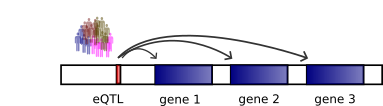
\includegraphics[width=\textwidth]{fig/model1.png}
    \end{subfigure}
%
    \begin{subfigure}[]{0.95\textwidth}
        \textbf{b}
        \\
        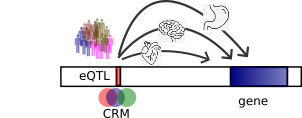
\includegraphics[width=\textwidth]{fig/model2.png}
    \end{subfigure}

    \caption{\textbf{Model of regulatory variant pleiotropy.} I have investigated three possible mechanisms of pleiotropy. \textbf{Left}, Pleiotropic variants have more eGenes that result in more functions and more phenotypes. This might arise from an enrichment of pleiotropic variants in splicing or 3' UTR regions. \textbf{Center}, I have also found that eGenes of pleiotropic variants are active in more etissues which result in more GWAS phenotypes. This might be explained from variants being bound by more transcription factors. \textbf{Left} Triplets of variant-eGene-eTissues are associated with more GWAS phenotypes, which directly affect the number of GWAS phenotypes. I have found that this might be explained by an enrichment of missense alleles.} \label{fig:beta}
%
\end{figure}
